%\newpage
% -----------------------------------------------------------------------
\chapter{Coursework}
%-----------------------------------------------------------------------
\section{Introduction}
A project will cover most of the topics from this course. At the end
of each chapter, there will be a set of exercises which are used to
strengthen the knowledge in software engineering. In addition, each
student will have the possibility to play around with the tools
demonstrated in this course.\\
For all the coursework, each student needs to have a computer
(Windows, OSX or Linux) with the possibility to install additional
software.

\subsection{Projects}
There are two projects available. The two projects are
developed for the following two courses:

\begin{itemize}
\item Gene Information Service (FHNW - Master Medical Informatics)
\item Raspberry Pi GPIO Web Application (FHNW - Master Automation Management)
\end{itemize}


\section{DNA}
DNA (deoxyribonucleic acid) is a long molecule that contains the
unique genetic code. Like a recipe book it holds the instructions for
making all the proteins in our bodies.
\begin{itemize}
\item DNA contains four bases:\\
adenine (A), cytosine (C), guanine (G) and thymine (T).
\item The sequence of these bases form the instructions in the genome.
\item DNA is a two-stranded molecule.
\item The bases on one strand of the DNA molecule pair together with
complementary bases on the opposite strand of DNA.\\
The bases always pair together in the same way, A with T, C with G.
\item Each strand of DNA has a beginning and an end,
called \verb|5'| (five prime) and \verb|3'| (three prime) respectively.
\end{itemize}

\begin{centering}
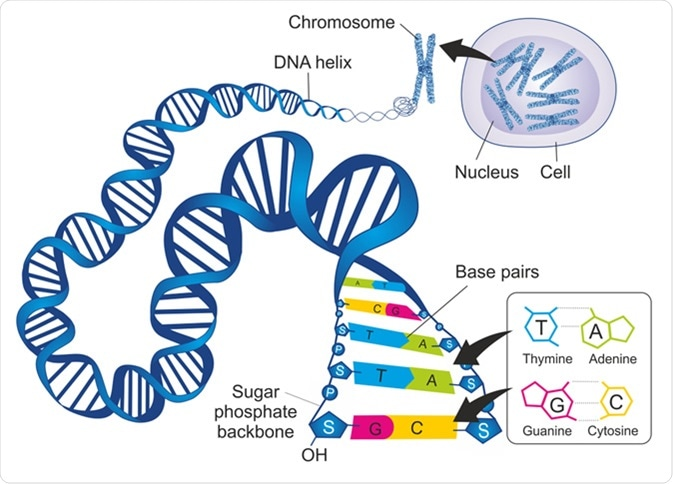
\includegraphics[width=360pt]{images/coursework/dna.jpeg}\\
(Source: https://www.news-medical.net)
\end{centering}

\section{Genome Assembly}
Genome assembly is the process of taking a large number of short
DNA sequences and putting them back together to create a representation
of the original DNA Sequence.\\
There are two types of genome assembly:
\begin{itemize}
\item De novo assembly\\
Assembling short reads to create the original sequence, with
no prior knowledge of the source DNA sequence length, layout or composition.\\
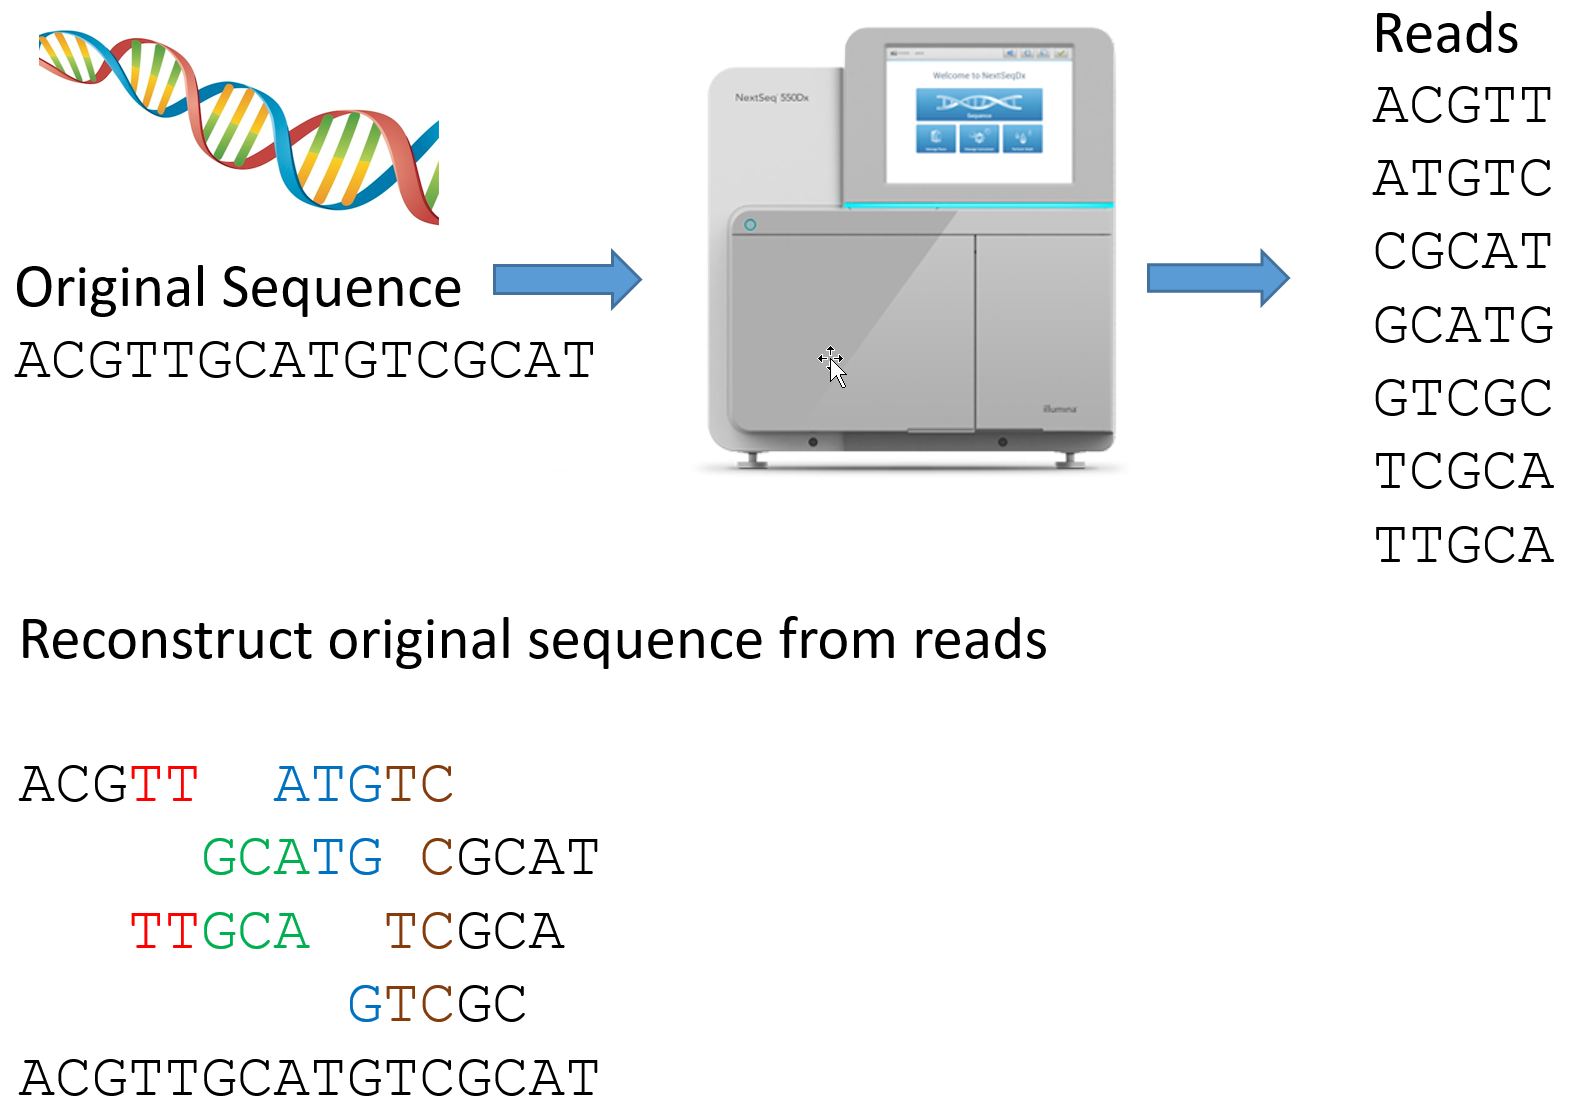
\includegraphics[width=300pt]{coursework/genomeassembly}
\item Reference mapping assembly\\
assembling reads against an existing reference sequence, building a sequence
that is similar but not necessarily identical to the reference sequence
\end{itemize}

\section{Software system}
The software system created in this course will be a Java based
web application, which is able to paste (or upload) a set of
reads and perform a de novo genome assembly. The user interface could
look like the following one:
